\section{Single axis experiments}
The second integrator model and its inputs-memory model will be studied over a single axis.
In order to compare the different abstractions and their sizes, we will find the smallest feasible solution for our controller synthesis problem.

We will compare the input extended state abstraction with the direct abstraction of the model (without input extended state).

\comment{Things to explains:
\begin{itemize}
\item Speed profiles (add the velocity commands)
\item Computation of the time
\end{itemize}
}

\subsection{Second integrator model with velocity feedback}
\begin{figure}[!ht]
	\begin{minipage}[b]{0.5\textwidth}
  		\centering
  		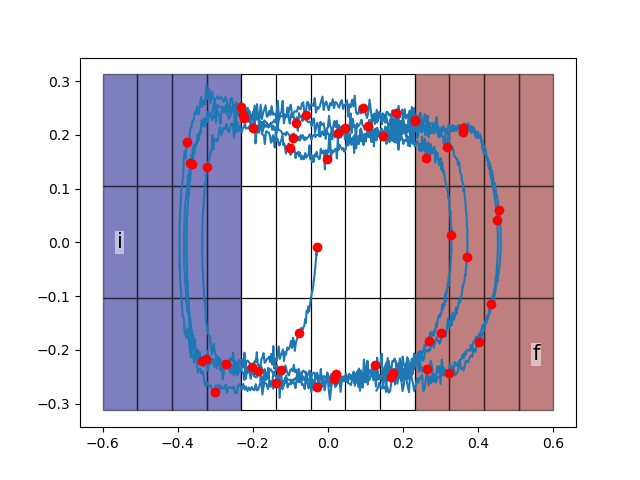
\includegraphics[width=0.9\linewidth]{double_1D}
	  	\caption{Trajectory in the 2D environment.}
	  	\label{double_1D}
  \end{minipage}
	\begin{minipage}[b]{0.5\textwidth}
  		\centering
  		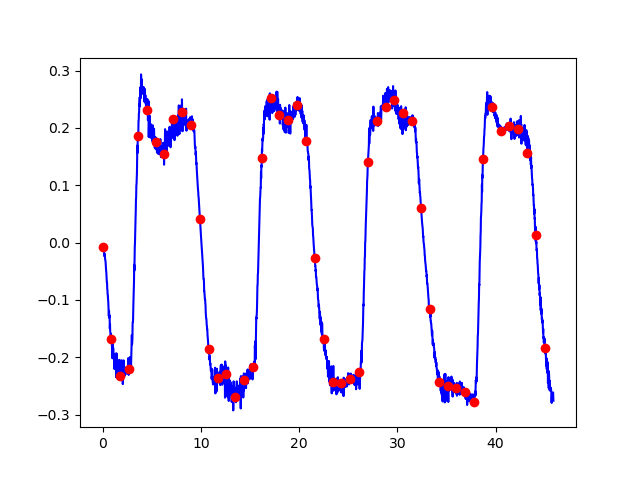
\includegraphics[width=0.9\linewidth]{double_1D_vel}
	  	\caption{Velocity profile.}
	  	\label{double_1D_vel}
  \end{minipage}
  \caption{Trajectory and velocity profile of the double integrator model. The agent is trying to achieve 'go infinity often to i and f'.}
\end{figure}

%% SELF LOOPS ON THE VELOCITY AXIS
The discretization of the state space is chosen to allow self loops during the steady states.
Regardless of the escape time property for the second integrator model, the self loops are not acceptable during transient state. If the transient state evolution is not observed in the case of the second integrator then the abstraction will be stuck in the transient state which make the abstraction not controllable.
\comment{plot the noise}

In figure \ref{double_1D_vel}, the position of the agent at $x\approx0.4$ is clearly going backward. This show that this model is not usable with the single integrator model.

\subsection{Model with $\Ninputs= 1$ memory}
\begin{figure}[!ht]
	\begin{minipage}[b]{0.5\textwidth}
  		\centering
  		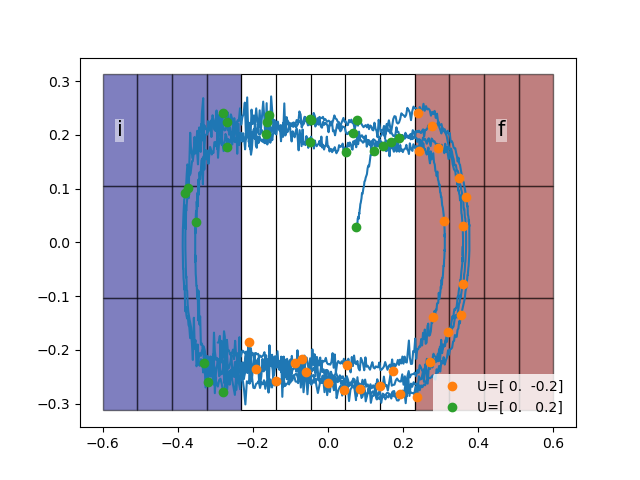
\includegraphics[width=\linewidth]{double_reduced_1D}
	  	\label{double_reduced_1D}
  \end{minipage}
	\begin{minipage}[b]{0.5\textwidth}
  		\centering
  		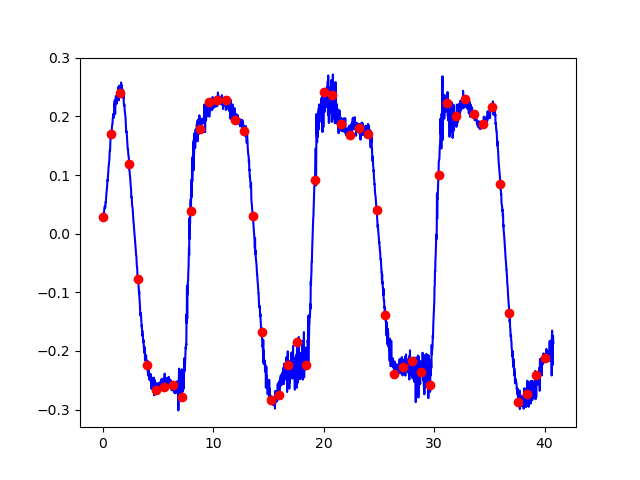
\includegraphics[width=\linewidth]{double_reduced_1D_vel}
	  	\label{double_reduced_1D_vel}
  \end{minipage}
  \caption{Trajectory and velocity profile of the double integrator 1-input memory model. The agent is trying to achieve 'go infinity often to i and f'.}
\end{figure}

\begin{figure}[!ht]
  	\centering
	\includestandalone[width=0.5\textwidth]{noise_plot}
  	\label{double_reduced_1D_noise}
  	\caption{The admissible noise of the abstraction have higher magnitudes for the high frequencies. The first plot correspond to the trajectory of the quad, the second is a plot of the noise (plain line) with noise upper and lower bounds (in simple dashed lines) and the upper and lower noise bounds used in the model (double dashed line).}
\end{figure}

%% Justification that this model is relevant
In our setup, the sampling time of model is ${\Delta t = 0.7s}$ and the timing constants of the unobserved system is $\tau_r = {\nicefrac{1}{k} = 0.5s}$. This is relevant to use this input memory model as the internal dynamics of the quadricopter are close to the sampling time of the sampling time.

%% SELF LOOPS:
% there is no self loops during the transiant state anymore
% there are still there for the steady states
% pourquoi mon model est controllqble ici et pas le second integrator
Every transition in the FTS encapsulate the knowledge of $\Ninputs +1$ control actions ($\Ninputs$ from the state and 1 from the transition). This correspond to the knowledge of the previous $(\Ninputs +1)\dt$ of the input function. 
In our models, the dynamics of the quadricopter are faster than $(\Ninputs +1)\dt = 1.4>0.5s$.
So every transition is able to predict the state of the unobserved system further than the time needed to vanished the transient state.
This result in the suppression of all the self loops due to the transient states that were present in the second integrator model.
The abstraction is smaller but as expressive (in term of controllability) than the second integrator model.

%% NOISE
% the noise is bigger than the modelled noise
Figure \ref{double_reduced_1D_noise} show an admissible noise sequence.
High frequencies of the noise can have a bigger magnitude than the modelled one. 
In the case of the second integrator model, any noise sequence with higher frequency might bring the model to take a nonexistant transition.

%% Size of the abstraction

%% Conclusion size of the abstraction

\subsection{Model with $\Ninputs=0$ memory} \label{sec:single_int}
\begin{figure}[!ht]
	\begin{minipage}[b]{0.5\textwidth}
  		\centering
  		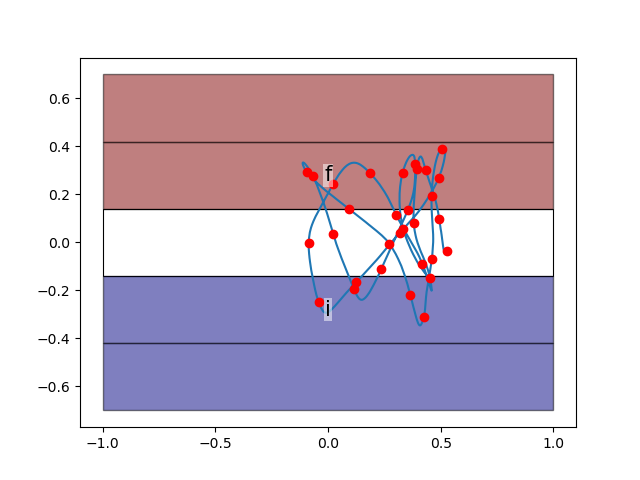
\includegraphics[width=0.9\linewidth]{simple_1D}
	  	\label{simple_1D}
  \end{minipage}
	\begin{minipage}[b]{0.5\textwidth}
  		\centering
  		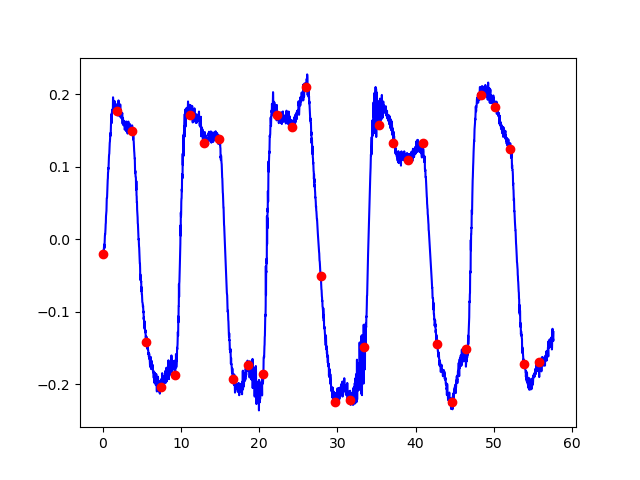
\includegraphics[width=0.9\linewidth]{simple_1D_vel}
	  	\label{simple_1D_vel}
  \end{minipage}
  \caption{Trajectory and velocity profile of the simple integrator model with self loops. The agent is trying to achieve 'go infinity often to i and f'.}
\end{figure}

\begin{figure}[!ht]
	\begin{minipage}[b]{0.5\textwidth}
  		\centering
  		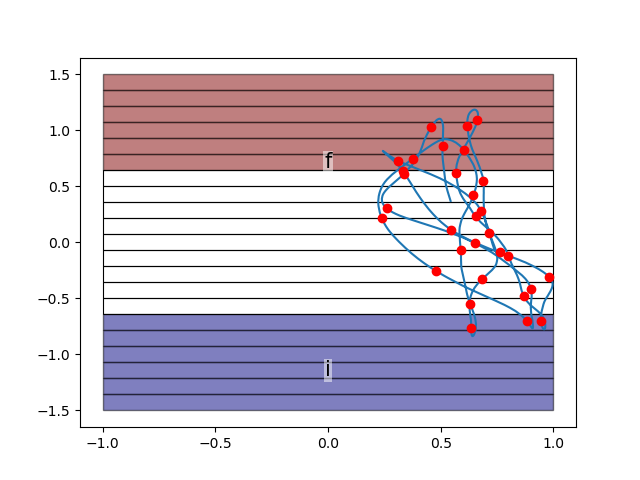
\includegraphics[width=0.9\linewidth]{simplenosl_1D}
	  	\label{simplenosl_1D}
  \end{minipage}
	\begin{minipage}[b]{0.5\textwidth}
  		\centering
  		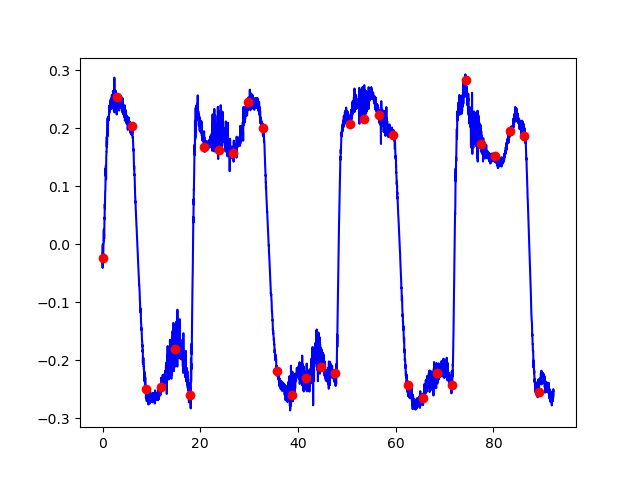
\includegraphics[width=0.9\linewidth]{simplenosl_1D_vel}
	  	\label{simplenosl_1D_vel}
  \end{minipage}
  \caption{Trajectory and velocity profile of the simple integrator model without self loops. The agent is trying to achieve 'go infinity often to i and f'.}
\end{figure}

\comment{Show the generated plans!}

This model is equivalent to the single integrator model.
We have been illustrating the advantages of self loops by doing one experiment with self loops and another experiment without self loops.
The FTS created without self loops needs to have a much finer discretization of the state space.
Whereas in the FTS with self loops, the constraint on the minimal size of the state space discretization is only that the transient state on the velocity must counteract the effect of the noise.

\subsection{Comparison of the two results}
\comment{
\begin{itemize}
\item compute the minimal number of states so that the model is usable (ie controllable)
\item compute the branching factor, the precision etc...
\item compute the amplitude of the noise in permanent state
\end{itemize}
}

Try to do it for different $\Delta n_u$, show that it does decrease the complexity for $\Delta n_u = 1$. Talk about the case $\Delta n_u = 0$ which correspond to the single integrator case (see part \ref{sec:single_int}).

Comparison to the double integrator case, show how the noise is evolving. Compare the size of the successors between the case where the discretization of the unobserved state (velocity in this case) is lower than the steady state of the unobserved state for a stable sequence. Basically, in one case, the size of the successors is growing (expansion of the successors) in the input memory approach, the size of the successors is reducing (but is bigger than the other one).


\comment{Try to show the 2 abstractions on top of each other to visualize what happened after the reduction}.

\paragraph{Sensitivity to noise}:
Please note that this model is less sensible to the noise on velocity as only the position is observed.
We have been noticing that this model was much easier to use thanks to this property.

\subsection{Discussion over the different models}
TODO


